%%%%%%%%%%%%%%%%%%%%%%%%%%%%%%%%%%%%%%%%%%%%%%%%%%%%%%%%%%%%%%%%%%%%%%%%%%%%%%%%%%%%%%%%%
% Khóa luận tốt nghiệp/Tiểu luận 
% LaTeX Template
% Phiên bản 1.0 (tạo ra ngày 05/10/2022)
% Edited &Modified by VietNC ngày 12/12/2022
%
% Template này có thể được download tại:
% https://github.com/vietnc/HUS-template
% https://github.com/cpc1996/HUS-Dissertation-Template
% 
%
% Phiên bản 1.0 được chỉnh sửa bởi:
% Công Phương Cao (congphuongcao_t59@hus.edu.vn)
% Nguyễn Cảnh Việt (vietncp@gmail.com)
% Nguyễn Tiến Cường (ngtiencuong@gmail.com)
%
% Template được tham khảo từ một phiên bản template của:
% Steve Gunn (http://users.ecs.soton.ac.uk/srg/softwaretools/document/templates/)
% Sunil Patel (http://www.sunilpatel.co.uk/thesis-template/)
%
%%%%%%%%%%%%%%%%%%%%%%%%%%%%%%%%%%%%%%%%%%%%%%%%%%%%%%%%%%%%%%%%%%%%%%%%%%%%%%%%%%%%%%%%%
%----------------------------------------------------------------------------------------
%	(KHÔNG CHỈNH SỬA PHẦN NÀY)
%
%	PHẦN 1: CÁC PACKAGE CƠ BẢN VÀ CÁC TÙY CHỈNH VĂN BẢN
%----------------------------------------------------------------------------------------
%----------------------------------------------------------------------------------------
%	(KHÔNG CHỈNH SỬA PHẦN NÀY)
%
%	PHẦN 1: CÁC PACKAGE CƠ BẢN VÀ CÁC TÙY CHỈNH VĂN BẢN
%----------------------------------------------------------------------------------------

\documentclass[
12pt,
oneside,
english,
doublespacing,
nolistspacing,
liststotoc,
parskip,
headsepline,
chapterinoneline,
]{MastersDoctoralThesis}

% \usepackage[utf8]{inputenc} 
\usepackage[utf8]{vietnam} 
%\usepackage[T1]{fontenc}

\usepackage{mathptmx}
\usepackage{amsmath}
\allowdisplaybreaks

%https://www.overleaf.com/learn/latex/Biblatex_citation_styles
%\usepackage[backend=bibtex,style=authoryear,natbib=true]{biblatex}
\usepackage[backend=bibtex,style=numeric,citestyle=ieee,natbib=true]{biblatex}

\addbibresource{main.bib}

\usepackage[autostyle=true]{csquotes}


%----------------------------------------------------------------------------------------
%	PHẦN 2: CÁC PACKAGE BỔ TRỢ THÊM VÀO TRONG QUÁ TRÌNH BIÊN SOẠN
%----------------------------------------------------------------------------------------

\RequirePackage{setlst}		% Liệt kê/trích dẫn code

\usepackage{multirow}
\usepackage{subfigure}
\usepackage[fontsize=13pt]{scrextend}

%https://www.sascha-frank.com/latex-font-size.html
%https://tex.stackexchange.com/questions/103286/how-to-change-section-subsection-font-size
\usepackage{titlesec}

\titleformat{\section}
{\normalfont\fontsize{13}{13}\bfseries}{\thesection}{1em}{}

\titleformat{\subsection}
{\normalfont\fontsize{13}{13}\bfseries\itshape}{\thesubsection}{1em}{}

%https://tex.stackexchange.com/questions/351961/how-to-indent-code-in-beginverbatim
\usepackage{fancyvrb} 		% Fancy Verbatim
\fvset{tabsize=4,vspace=0pt,fontsize=\footnotesize}

\usepackage{longtable} 		% Bảng dài - Long table

\usepackage[figuresright]{rotating} % Bảng ngang - Sideways table
\usepackage{tabularx}

\usepackage{fontawesome5} 	% Các biểu tượng, ký hiệu đặc biệt

\usepackage{tikz} 			% Vẽ hình
\usepackage{indentfirst}
\setlength{\parindent}{0.5cm}	%Thut dau dong cho doan van
\setlength{\parskip}{1.4ex plus 0.5ex minus 0.3ex}		% Tạo khoảng trống giữa 2 đoạn văn %spacing between two paragraph

\usetikzlibrary{calc}
%----------------------------------------------------------------------------------------
%	PHẦN 3: THÔNG TIN VỀ Khóa luận tốt nghiệp/Tiểu luận (THESIS INFORMATION)
% 	Điền thông tin của các bạn trong file(2.thesis-information) này 
%----------------------------------------------------------------------------------------
%----------------------------------------------------------------------------------------
%	PHẦN 3: THÔNG TIN VỀ Khóa luận tốt nghiệp/Tiểu luận (THESIS INFORMATION)
%----------------------------------------------------------------------------------------
\author{NGUYỄN CÔNG DŨNG \\TRẦN QUỐC KHANG \\NGUYỄN TRỌNG SƠN} 			% Ví dụ: "Nguyễn Thị Thu Thảo"
\thesistitle{ỨNG DỤNG THUẬT TOÁN TÌM KIẾM TRONG ĐỒ THỊ TÌM KIẾM ĐƯỜNG ĐI TRONG MÊ CUNG} % Ví dụ: "Nghiên cứu chế tạo và tính chất quang học của vật liệu nano LaF3:Sm3+"

\supervisor{Phạm Huy Thông} 	% Ví dụ: "PGS. TS. Nguyễn Ngọc Long"
\supervisorr{} 	% Tên này nếu không có thì để trống!

\field{CẤU TRÚC DỮ LIỆU VÀ GIẢI THUẬT} 					% Ví dụ: "Ngành Vật lý", "Ngành Hóa học", v.v.
\program{NGÀNH KỸ THUẬT ĐIỆN TỬ VÀ TIN HỌC} 			% Ví dụ: "Chương trình đào tạo chuẩn", "Chương trình đào tạo cử nhân tài năng", v.v.
\doctype{BÁO CÁO} % Điền vào đây: "Khóa luận tốt nghiệp đại học hệ chính quy" hoặc "Tiểu luận"

\university{\href{http://hus.vnu.edu.vn}{TRƯỜNG ĐẠI HỌC KHOA HỌC TỰ NHIÊN}}
\department{\href{http://hus.vnu.edu.vn/gioi-thieu/co-cau-to-chuc/khoa-truc-thuoc/khoa-vat-ly.html}{KHOA VẬT LÝ}}

\AtBeginDocument{
	\hypersetup{pdftitle=\ttitle}
	\hypersetup{pdfauthor=\authorname}
}

%----------------------------------------------------------------------------------------------------------------------------------------
\begin{document}
\lstset{style=codeC}	% Thiết lập ngôn ngữ C/C++ là ngôn ngữ mặc định cho phần liệt kê souce code của cả bài
\frontmatter 			% Sử dụng hệ thống đánh số La Mã (i, ii, iii, iv...) cho những trang trước phần mục lục
\pagestyle{plain} 
%----------------------------------------------------------------------------------------
%	(KHÔNG CHỈNH SỬA PHẦN NÀY)%
%	PHẦN 4: TRANG TIÊU ĐỀ/TRANG BÌA (TITLE PAGE)
%----------------------------------------------------------------------------------------
% TRANG BÌA CHÍNH:
%----------------------------------------------------------------------------------------
%	(KHÔNG CHỈNH SỬA PHẦN NÀY)
%
%	Phần 6: TRANG TIÊU ĐỀ/TRANG BÌA (TITLE PAGE)
%----------------------------------------------------------------------------------------

% TRANG BÌA CHÍNH:
\begin{titlepage}
	\begin{tikzpicture}[overlay,remember picture]
		\draw [line width=3pt]
		($ (current page.north west) + (2.0cm,-2.0cm) $)
		rectangle
		($ (current page.south east) + (-1.5cm,1.8cm) $);
		\draw [line width=1pt]
		($ (current page.north west) + (2.15cm,-2.15cm) $)
		rectangle
		($ (current page.south east) + (-1.65cm,1.95cm) $); 
	\end{tikzpicture}
	\begin{center}
		
		\vspace{-.04\textheight}
%		\noindent\scshape 			% By CPC
		\noindent 			% Edit by VietNC
		\large \, \href{https://www.vnu.edu.vn/home/}{ĐẠI HỌC QUỐC GIA HÀ NỘI}\\
		\vspace{-0.25cm}{\large \MakeUppercase \univname}\\
		\vspace{-0.25cm}{\large \bfseries \MakeUppercase \deptname}\\[0.5cm]
		
\includegraphics{Logo/Logo_HUS_notext_nocolor}
		
		\vspace{1.0cm}
		
		{\large \MakeUppercase \authorname}
		
		\vspace{2.5cm}
		
		{\Large \bfseries \MakeUppercase\ttitle\par}
		
		\vspace{2.5cm}
		
		{\normalsize \docname\\ \fieldname\\ (\progname)\\}
		
		\vfill
		
		\textbf{Hà Nội - \the\year{}}
	\end{center}
\end{titlepage}


% TRANG BÌA PHỤ:
%----------------------------------------------------------------------------------------
%	(KHÔNG CHỈNH SỬA PHẦN NÀY)
%
%	Phần 6: TRANG TIÊU ĐỀ/TRANG BÌA (TITLE PAGE)
%----------------------------------------------------------------------------------------

% TRANG BÌA PHỤ:
\begin{titlepage}
	\begin{tikzpicture}[overlay,remember picture]
		\draw [line width=3pt]
		($ (current page.north west) + (2.0cm,-2.0cm) $)
		rectangle
		($ (current page.south east) + (-1.5cm,1.8cm) $);
		\draw [line width=1pt]
		($ (current page.north west) + (2.15cm,-2.15cm) $)
		rectangle
		($ (current page.south east) + (-1.65cm,1.95cm) $); 
	\end{tikzpicture}
	\begin{center}
		
		\vspace{-.04\textheight}
%		\noindent\scshape    % By CPC
		\noindent                  % Edit by VietNC
		\large \, \href{https://www.vnu.edu.vn/home/}{ĐẠI HỌC QUỐC GIA HÀ NỘI}\\
		\vspace{-0.25cm}{\large \MakeUppercase \univname}\\
		\vspace{-0.25cm}{\large \bfseries \MakeUppercase \deptname}\\[0.5cm]
		
\includegraphics{Logo/Logo_HUS_notext}
		
		\vspace{1.0cm}
		
		{\large \MakeUppercase \authorname}
		
		\vspace{2.5cm}
		
		{\Large \bfseries \MakeUppercase\ttitle\par}
		
		\vspace{2.5cm}
		
		{\normalsize \docname\\ \fieldname\\ (\progname)\\}
		
		\vspace{2.5cm}
		
		\begin{minipage}[t]{0.49\textwidth}
			\begin{flushright} \large \bfseries
				Giảng viên hướng dẫn:\;
			\end{flushright}
		\end{minipage}
		\begin{minipage}[t]{0.5\textwidth}
			\begin{flushleft} \large \bfseries
				\supname\\
				\supnamee
			\end{flushleft}
		\end{minipage}
		
		\vfill
		
		\textbf{Hà Nội - \the\year{}}
	\end{center}
\end{titlepage}


%----------------------------------------------------------------------------------------
%	PHẦN 5: DANH NGÔN (QUOTES)
%----------------------------------------------------------------------------------------
%\vspace*{0.2\textheight}

%\noindent\enquote{\itshape 
%	Cái tôi và sự hiểu biết tỷ lệ nghịch với nhau. Hiểu biết càng nhiều cái tôi càng bé. Hiểu biết càng ít, cái tôi càng to.
%}\bigbreak

%\hfill Albert Einstein
%----------------------------------------------------------------------------------------
%	PHẦN 6: LỜI CẢM ƠN (ACKNOWLEDGEMENTS)
%	Các bạn ghi lời cảm ơn vào file(5.ack) này.
%----------------------------------------------------------------------------------------
%%----------------------------------------------------------------------------------------
%	PHẦN 6: LỜI CẢM ƠN (ACKNOWLEDGEMENTS)
%----------------------------------------------------------------------------------------

\begin{acknowledgements}
	\addchaptertocentry{\acknowledgementname}
	\thispagestyle{empty}
	Trong quá trình nghiên cứu và hoàn thành bài tập cuối kỳ, chúng em đã nhận được sự định hướng, giúp đỡ, các ý kiến đóng góp quý báu và các lời động viên của các thầy cô giáo, gia đình và bạn bè.
	Chúng em xin gửi lời cảm ơn sâu sắc tới thầy Th.S Nguyễn Cảnh Việt đã tận tình hướng dẫn và giúp đỡ em trong quá trình nghiên cứu và thực hiện bài báo cáo này. Thầy không chỉ dạy em những kiến thức không chỉ về chuyên ngành, về môn học, mà còn hướng dẫn, chỉ bảo về cách sống, tác phong làm việc,…Những điều thầy đã dạy quả thật rất bổ ích và em tin chắc rằng nó sẽ giúp em rất nhiều trong cuộc sống sau này.
	Trong quá trình học tập cũng như thực hiên bài báo cáo, khó tránh khỏi những sai sót không đáng có, rất mong Thầy thông cảm và bỏ qua. Ngoài ra bài báo cáo còn rất nhiều chỗ thiếu sót, chúng em rất mong nhận được những ý kiến đóng góp của Thầy để giúp em có thể hoàn thiện và chuẩn bị tốt hơn cho những bài báo cáo tiếp theo.\\
	Chúng em xin chân thành cảm ơn!\\
	
	\hfill Sinh viên Ngô Đăng Huy \& Nguyễn Trọng Sơn
\end{acknowledgements}
%----------------------------------------------------------------------------------------
%	(KHÔNG CHỈNH SỬA PHẦN NÀY)
%
%	PHẦN 7: MỤC LỤC (LIST OF CONTENTS/FIGURES/TABLES PAGES)
%	ĐẶT KHOẢNG CÁCH GIŨA CÁC TIÊU ĐỀ CỦA PHẦN 7
%----------------------------------------------------------------------------------------
\begin{spacing}{1.15}
	\tableofcontents 	% In ra mục lục chính
\end{spacing}

\begin{spacing}{1.15}
	\listoffigures 		% In ra danh sách hình vẽ
\end{spacing}

%\begin{spacing}{1.15}
%	\listoftables		% In ra danh sách bảng
%\end{spacing}

%----------------------------------------------------------------------------------------
%	PHẦN 8: DANH SÁCH TÊN VIẾT TẮT (ABBREVIATIONS)
%
%	Các từ viết tắt các bạn ghi ở đây
%----------------------------------------------------------------------------------------
%\begin{abbreviations}{ll} % Thêm danh sách tên viết tắt (dưới dạng một bảng có 2 cột)
%
%\textbf{Tx} & \textbf{N}hiệt \textbf{Đ}ộ \textbf{C}ực \textbf{Đ}ại\\
%\textbf{Tm} & \textbf{N}hiệt \textbf{Đ}ộ \textbf{C}ực \textbf{T}iểu\\
%
%\end{abbreviations}
%----------------------------------------------------------------------------------------
%	PHẦN 9: CÁC HẰNG SỐ VẬT LÝ/THÔNG SỐ KĨ THUẬT (PHYSICAL CONSTANTS/OTHER DEFINITIONS)
%----------------------------------------------------------------------------------------
%\begin{constants}{lr@{${}={}$}l} % Thêm danh sách các hằng số (dưới dạng một bảng có 3 cột)
%
%%	Lệnh \SI{}{} được cung cấp bởi gói siunitx, hãy đọc tài liệu hướng dẫn để biết cách sử dụng nó
%
%%	Tên hằng số 	 & $Biểu tượng$	& $Hằng số$ cùng với đơn vị\\
%	Vận tốc ánh sáng & $c_{0}$		& \SI{2.99792458e8}{\meter\per\second} (chính xác)\\
%
%\end{constants}
%----------------------------------------------------------------------------------------
%	PHẦN 10: DANH SÁCH KÝ HIỆU (SYMBOLS)
%----------------------------------------------------------------------------------------

%\begin{symbols}{lll} % Thêm danh sách các ký hiệu (dưới dạng một bảng có 3 cột)
%
%%   Ký hiệu	& Ý nghĩa		& Đơn vị \\
%	$a$		& khoảng cách	& \si{\meter} \\
%	$P$		& công suất		& \si{\watt} (\si{\joule\per\second}) \\
%
%	\addlinespace % Khoảng cách để phân biệt giữa ký hiệu Latin với ký hiệu La Mã
%
%	$\omega$ & tần số góc	& \si{\radian} \\
%
%\end{symbols}

%----------------------------------------------------------------------------------------
%	(KHÔNG CHỈNH SỬA PHẦN NÀY)
%
%	PHẦN 11: LỜI ĐỀ TẶNG (DEDICATION)
%----------------------------------------------------------------------------------------

%\dedicatory{Dành tặng/Dành cho/Gửi tới\ldots} 


%----------------------------------------------------------------------------------------
%	PHẦN 12: NỘI DUNG/CÁC CHƯƠNG Khóa luận tốt nghiệp/Tiểu luận (THESIS CONTENT - CHAPTERS)
%----------------------------------------------------------------------------------------

\mainmatter % Bắt đầu đánh số trang (1,2,3...)

\pagestyle{plain}

% Hãy thêm những chương (chapter) của khóa luận/tiểu luận vào thư mục Chapters
% Hãy bỏ chú thích những dòng nếu bạn đã bổ sung những chương vào


\chapter*{MỞ ĐẦU} % Tên của chương
\addcontentsline{toc}{chapter}{MỞ ĐẦU} % Thêm tên chương vào mục lục

\label{Chapter6} % Để trích dẫn chương này ở chỗ nào đó trong bài, hãy sử dụng lệnh \ref{Chapter0} 

%----------------------------------------------------------------------------------------
Thuật toán tìm kiếm đường đi trong mê cung là một trong những bài toán cơ bản và thường được sử dụng trong môn cấu trúc dữ liệu và giải thuật. Việc tìm kiếm đường đi trong mê cung là một ví dụ điển hình để giới thiệu các thuật toán tìm kiếm và các khái niệm cơ bản như đồ thị, quy hoạch động và các kỹ thuật tối ưu.

Mô phỏng thuật toán tìm kiếm đường đi trong mê cung giúp sinh viên hiểu và tự tìm hiểu các giải thuật, tạo cảm hứng và khai thác triệt để các kiến thức được học. Không chỉ dừng lại ở các mô tả trên lý thuyết, mô phỏng các thuật toán tìm kiếm đường đi trong mê cung giúp sinh viên biết cách thực hiện áp dụng vào các bài tập trên thực tế.

Với sức mạnh của công nghệ, mô phỏng thuật toán tìm kiếm đường đi trong mê cung càng trở nên dễ dàng hơn bằng việc sử dụng các công cụ và thư viện phần mềm để tạo ra một môi trường mô phỏng và thực hiện việc đánh giá các thuật toán tìm kiếm đường đi. Điều này giúp cho môn học cấu trúc dữ liệu và giải thuật có thể được học một cách trực quan và hiệu quả hơn.

% Chương 1

\chapter{TÌM KIẾM ĐƯỜNG ĐI TRONG MÊ CUNG} % Tên của chương

\label{Chapter1} % Để trích dẫn chương này ở chỗ nào đó trong bài, hãy sử dụng lệnh \ref{Chapter1} 

%----------------------------------------------------------------------------------------

% Định nghĩa một số lệnh cần thiết để điều chỉnh định dạng cho một số nội dung nhất định trong bài
\newcommand{\keyword}[1]{\textbf{#1}}
\newcommand{\tabhead}[1]{\textbf{#1}}
\newcommand{\code}[1]{\texttt{#1}}
\newcommand{\file}[1]{\texttt{\bfseries#1}}
\newcommand{\option}[1]{\texttt{\itshape#1}}

%----------------------------------------------------------------------------------------
\section{Giới thiệu}
Mô phỏng tìm đường đi trong mê cung là một phương pháp để tìm kiếm đường đi từ một điểm bắt đầu tới một điểm kết thúc trong một mê cung. Phương pháp này áp dụng các thuật toán tìm kiếm đường đi, như DFS, BFS, A*,... để tìm ra đường đi ngắn nhất hoặc đường đi tối ưu nhất trong mê cung.

Mô phỏng tìm đường đi trong mê cung thường được sử dụng trong lĩnh vực trò chơi điện tử để tạo ra các trò chơi dạng mê cung và giải quyết bài toán đi qua mê cung. Ngoài ra, nó còn được ứng dụng trong các lĩnh vực như điều khiển tàu thủy, máy tính thông minh,...

Trong quá trình mô phỏng, các tường, các đường đi và các điểm đích sẽ được tạo ra. Sau đó, người dùng sẽ nhập vào điểm bắt đầu và điểm kết thúc, và trải nghiệm quá trình tìm đường đi thông qua các thuật toán tìm kiếm đường đi được tích hợp trong mô phỏng.

Mô phỏng tìm đường đi trong mê cung giúp người dùng hiểu rõ hơn về cách thức hoạt động của các thuật toán tìm kiếm đường đi và cách chúng giải quyết bài toán đi qua mê cung.



\section{Mô tả}
Việc mô phỏng thuật toán tìm kiếm đường đi trong mê cung thường bao gồm các bước sau:

\begin{enumerate}
	\item Tạo ra môi trường mê cung: Đầu tiên, chúng ta cần tạo ra một môi trường mê cung. Điều này có thể được thực hiện bằng cách sử dụng các thuật toán tạo ra mê cung có sẵn, hoặc có thể sử dụng các công cụ thiết kế môi trường để tự tạo ra một mê cung.
	\item Xác định các điểm bắt đầu và kết thúc: Sau khi tạo ra mê cung, chúng ta cần xác định các điểm bắt đầu và kết thúc. Điểm bắt đầu là nơi mà thuật toán bắt đầu tìm kiếm đường đi, trong khi điểm kết thúc là mục tiêu của chúng ta trong quá trình tìm kiếm đường đi.
	\item Chọn thuật toán tìm kiếm đường đi: Nhiều thuật toán khác nhau có thể được sử dụng để tìm kiếm đường đi trong mê cung, bao gồm DFS (đi sâu trước), BFS (đi rộng trước), A* và nhiều thuật toán khác. Tùy thuộc vào mục đích và yêu cầu của ứng dụng, chúng ta nên chọn thuật toán tìm kiếm thích hợp nhất để đạt được kết quả tốt nhất.
	\item Thực hiện thuật toán tìm kiếm đường đi: Sau khi chọn thuật toán, chúng ta sẽ thực hiện nó để tìm kiếm đường đi từ điểm bắt đầu đến điểm kết thúc. Trong quá trình này, thuật toán sẽ di chuyển qua từng ô trong mê cung, theo các quy tắc của thuật toán được chọn và đưa ra quyết định để di chuyển sang ô tiếp theo.
	\item Hiển thị kết quả: Khi thuật toán tìm kiếm đường đi hoàn tất, chúng ta sẽ hiển thị kết quả tìm được cho người dùng, bao gồm đường đi từ điểm bắt đầu đến điểm kết thúc và độ dài của đường đi.
\end{enumerate}


Các bước này sẽ giúp chúng ta thực hiện việc mô phỏng thuật toán tìm kiếm đường đi trong mê cung một cách đơn giản và dễ hiểu. Việc mô phỏng này giúp người dùng hiểu rõ hơn về nguyên lý hoạt động của các thuật toán tìm kiếm đường đi và cách kết hợp chúng để tìm kiếm đường đi tối ưu trong một mê cung.








% Chương 2

\chapter{THUẬT TOÁN TÌM KIẾM} % Tên của chương

\label{Chapter2} % Để trích dẫn chương này ở chỗ nào đó trong bài, hãy sử dụng lệnh \ref{Chapter2} 

%----------------------------------------------------------------------------------------
Thuật toán tìm kiếm theo chiều sâu và chiều rộng là hai thuật toán tìm kiếm mù
phổ biến, thường được sử dụng trong lý thuyết đồ thị. Chúng ta sẽ đi vào từng
thuật toán từ tư tưởng của thuật toán cho tới giả mã và bước đi trong thuật toán để
làm rõ hơn cách thức hoạt động của thuật toán. Trong quá trình tìm hiểu ta sẽ nhận
thấy chúng có nhiều điểm tương đồng trong cách thực hiện, nhưng cách tổ chức thì
khác nhau. Với mỗi thuật toán ta sẽ đưa ra ưu nhược điểm của chúng để có thể sử
dụng chúng phù hợp hơn theo những yêu cầu riêng của bài toán đầu vào.

\section{Thuật toán tìm kiếm theo chiều sâu - Depth First Search (DFS)} 
Trước tiên ta sẽ đi vào tìm hiểu về thuật toán tìm kiếm theo chiều sâu (DFS) \cite{tl2}.
Thuật toán DFS là một quá trình duyệt hay tìm kiếm trên một cây hoặc một đồ thị.
Thuật toán DFS sẽ bắt đầu với một đỉnh gốc và phát triển sâu và xa nhất có thể của
mỗi nhánh. Để hiểu hơn ta sẽ đi vào từng phần trong thuật toán:

\subsection{Tư tưởng của thuật toán}
Với tư tưởng đi sâu vào từng nhánh, ta giả sử đầu vào của thuật toán là một đồ thị
G = (V,E). Coi s là đỉnh gốc của V, ta sẽ bắt đầu quá trình duyệt với s.Từ s ta sẽ đi
thăm tới đỉnh kề với s (giả sử ở đây là u0), từ u0 ta tiếp tục quá trình duyệt với các
đỉnh kề u0 (trừ các đỉnh đã thăm). Quá trình sẽ tiếp tục tới khi gặp đỉnh cần tìm
hoặc đi hết nhánh thì thực hiện lùi lại đỉnh trước đó.

Xét một cách tổng quát thì khi xét một đỉnh u0 ta sẽ có hai khả năng xảy ra:
\begin{itemize}
	\item Nếu như tồn tại đỉnh v0 kề với u0 mà chưa được thăm thì đỉnh v0 đó sẽ được
	đánh dấu để trở thành đỉnh đã thăm và quá trình tìm kiếm sẽ bắt đầu từ đỉnh v0
	đó.
	\item Ngược lại, nếu mọi đỉnh kề với u0 đều đã thăm thì ta sẽ quay lại đỉnh mà trước
	đó ta đến đỉnh u0 để tiếp tục quá trình tìm kiếm
\end{itemize}

Như vậy trong quá trình thăm đỉnh bằng thuật toán tìm kiếm theo chiều sâu, ta
nhận thấy ngay đỉnh càng thăm muộn thì sớm được duyệt trước (đây là cơ chế Last
In First Out) . Do đó ta có thể sử dụng thủ tục đệ quy hoặc sử dụng một danh sách
kiểu ngăn xếp để tổ chức cho quá trình duyệt của thuật toán. Dưới dây là minh họa
cho quá trình duyệt với một cây:

\begin{figure}[h!]
	\centering
	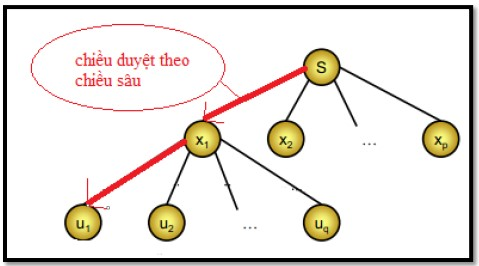
\includegraphics[width=0.8\textwidth]{
		Figures/figs/ThuTuDFS.jpg
	}
	\caption[Thứ tự duyệt của thuật toán DFS]{
		Thứ tự duyệt của thuật toán DFS 
	}
	\label{fig:hinha}
\end{figure}


Hình trên minh họa thứ tự duyệt của thuật toán tìm kiếm theo chiều sâu: ta nhận
thấy từ S sẽ thăm X1, tiếp tục tới u1 là kề với X1. Nếu u1 không phải đỉnh tìm và hết nhánh thì sẽ lùi về X1 để thăm u2. Do đó quá trình duyệt sẽ là: S $\to$ x1 $\to$ u1 $\to$ u2 $\to$ ... $\to$ uq $\to$ x2 $\to$ ...

\subsection{Giải thuật của thuật toán}
Xác định bài toán ta cần lấy ra input và output của bài toán như sau:
\begin{itemize}
	\item \textbf{Input:} đồ thị vào G=(V,E) với đỉnh gốc là s0(Trạng thái đầu)
	
	Tập đích Goal
	\item \textbf{Output:} một đường đi p từ s đến một đỉnh ftrong tập đích Goals
\end{itemize}

Thuật toán DFS có 2 cách để duyệt những đỉnh trong quá trình tìm kiếm đó là sử
dụng thủ tục đệ quy hoặc sử dụng ngăn xếp để lưu trữ các đỉnh sẽ duyệt tiếp đó. Ta
sẽ đi vào cách sử dụng ngăn xếp để lưu trữ các đỉnh.Ta có các bước cho quá trình
thực hiện thuật toán như sau:

\textbf{Bước 1:} khởi tạo
\begin{itemize}
	\item Các đỉnh đều ở trạng thái chưa đánh dấu, trừ đỉnh xuất phát s là đã đánh
	dấu.
	\item Một ngăn xếp S (Stack)ban đầu chỉ đưa vào có một phần tử là s. Bằng việc
	sử dụng ngăn xếp lưu các đỉnh ta sẽ duyệt sâu vào từng nhánh của đồ thị.
\end{itemize}

\textbf{Bước 2:} Lặp lại các bước sau cho đến khi ngăn xếp rỗng:
\begin{itemize}
	\item Nếu ngăn xếp rỗng, không thấy đỉnh đích, thông báo \textit{“không tìm thấy”},
	dừng.
	\item Ngăn xếp không rỗng, lấy u ra khỏi ngăn xếp, thông báo thăm u (bắt đầu
	duyệt đỉnh u, nếu lần đầu thì là u chính là s).
	\item Kiểm tra u có phải đỉnh đích t không:
		\subitem - Nếu đúng trả về u, dừng vòng lặp, chuyển sang bước 3.
		\subitem - Nếu không đúng thì tiếp tục duyệt.
	\item Xét tất cả các đỉnh v kề với u mà chưa được đánh dấu, với mỗi đỉnh v đó:
		\subitem - Đánh dấu v
		\subitem - Ghi nhận đường đi từ v đến u
		\subitem - Đẩy v vào ngăn xếp (v sẽ chờ được duyệt tại những bước sau)
\end{itemize}

\textbf{Bước 3:} Truy ngược lại đường đi (nếu có)

\subsection{Nhận xét}
\begin{itemize}
	\item Có thể có nhiều đường đi từ s $\to$ f, nhưng thuật toán DFS luôn trả về một
	đường đi có thứ tự từ điển nhỏ nhất.
	\item Quá trình tìm kiếm theo chiều sâu cho ta một cây DFS gốc s. Quan hệ chacon trên cây được định nghĩa là: nếu từ đỉnh u tới thăm đỉnh v thì u là nút
	cha của nút v. Hình dưới sẽ minh họa cho cây DFS tương ứng với đỉnh xuất
	phát s=1
\end{itemize}

\begin{figure}[h!]
	\centering
	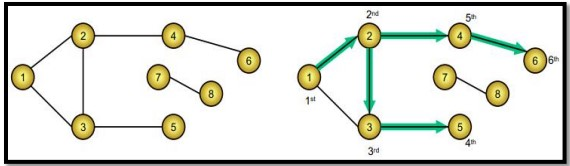
\includegraphics[width=0.8\textwidth]{
		Figures/figs/cayDFS_S1.jpg
	}
	\caption[Cây DFS với s = 1.]{
		Cây DFS với s = 1.
	}
	\label{fig:hinhb}
\end{figure}

\textbf{Ưu điểm}
\begin{itemize}
	\item Nếu bài toán có lời giải, phương pháp tìm kiếm theo chiều sâu đảm bảo tìm
	ra lời giải.
	\item Ký thuật tìm kiếm sâu tập trung vào đích, con người cảm thấy hài lòng khi
	các câu hỏi tập trung vào vấn đề chính.
	\item Do cách tìm của kỹ thuật này, nếu lời giải ở rất sâu, kỹ thuật sâu sẽ tiết
	kiệm thời gian
\end{itemize}

\textbf{Nhược điểm}
\begin{itemize}
	\item Tìm sâu khai thác không gian bài toán để tìm lời giải theo thuật toán đơn
	giản một cách cứng nhắc. Trong quá trình tìm nó không có thông tin nào để
	phát hiện lời giải. Nếu cọn nút ban đầu không thích hợp có thể không dẫn
	tới đích của bài toán.
	\item Không phù hợp với không gian bài toán lớn, kỹ thuật tìm kiếm sâu có thể
	không đi đến lời giải trong khoảng thời gian vừa phải (nếu cố định thời
	gian).
\end{itemize}

%----------------------------------------------------------------------------------------------------------------------------------------------------------------------------------------------------------------------------


\section{Thuật toán tìm kiếm theo chiều rộng (Breadth First Sreach)}
Tương tự thuật toán tìm kiếm DFS thì thuật toán BFS cũng là một thuật toán phổ
biến trong việc tìm kiếm trong đồ thị \cite{tl1}. Nhưng có đôi chút khác biệt về cách tổ chức
các đỉnh để duyệt so với thuật toán DFS. Do đó cách duyệt của BFS cũng trở nên
khác DFS. Để thấy sự khác nhau này ta sẽ đi vào tìm hiểu hơn vào thuật toán.

\subsection{Tư tưởng của thuật toán}
Ta giả sử đầu vào thuật toán là một đồ thị G = (V, E), ta sẽ phải thực hiện lập lịch
duyệt cho các đỉnh của đồ thị G. Việc duyệt các đỉnh sẽ được ưu tiên sao cho đỉnh
nào gần với nó nhất sẽ được duyệt trước. Tức là nó bắt đầu từ mức thấp nhất của
không gian bài toán, sẽ duyệt theo chiều từ trái sang phải hoặc ngược lại ở mức
tiếp theo, nếu không thấy lời giải ở mức này nó sẽ chuyển xuống mức kế để tiếp
tục...cứ như vậy đến khi tìm được lời giải (nếu có). Ta xét ví dụ sau:

Ví dụ : Bắt đầu ta thăm đỉnh S. Việc thăm đỉnh S sẽ phát sinh thứ tự duyệt những
đỉnh (x[1], x[2], .. ,x[p]) kề với S (những đỉnh gần S nhất). Khi thăm đỉnh x[1] sẽ
lại phát sinh yêu cầu duyệt những đỉnh (u[1], u[2], ..., u[q]) kề với x[1]. Nhưng rõ
ràng các đỉnh u này xa S hơn những đỉnh x nên chúng chỉ được duyệt khi tất cả các
đỉnh x đã được duyệt xong. Tức là thứ tự duyệt đỉnh sau khi đã thăm x[1] sẽ là :
(x[2], x[3], ..., x[p], u[1], u[2],..., u[q])

\begin{figure}[h!]
	\centering
	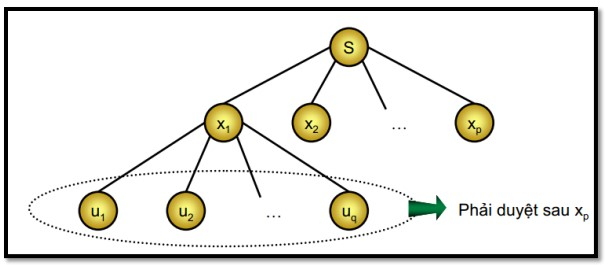
\includegraphics[width=0.8\textwidth]{
		Figures/figs/ThuTuBFS.jpg
	}
	\caption[Thứ tự duyệt thuật toán BFS]{
		Thứ tự duyệt thuật toán BFS
	}
	\label{fig:hinhc}
\end{figure}

\subsection{Giải thuật của thuật toán}
\begin{itemize}
	\item \textbf{Input:} cây đồ thị G= (V,E) với đỉnh gốc là $s_0$ ( trạng thái đầu)
	
	Tập đích Goals.
	\item \textbf{Output:} một đường đi p từ $n_0$ đến 1 đỉnh f trong tập Goals
\end{itemize}

Thuật toán sử dụng một cấu trúc dữ liệu là hàng đợi (Queue) để lưu trữ thông tin
trung gian trong quá trình tìm kiếm (ở đây dễ hiểu là các đỉnh kế tiếp đợi được
duyệt). Tương tự với tìm kiếm theo chiều sâu, các bước cho giải thuật tìm kiếm
theo chiều rộng như sau :

\textbf{Bước 1:} Khởi tạo
\begin{itemize}
	\item Các đỉnh đều ở trạng thái chưa đánh dấu, trừ đỉnh xuất phát s là đã đánh
	dấu.
	\item Một hàng đợi Q (tổ chức dạng hàng đợi Queue), ban đầu chỉ có một phần tử
	là s. Hàng đợi dùng để chứa các đỉnh sẽ được duyệt theo thứ tự ưu tiên
	chiều rộng.
\end{itemize}

\textbf{Bước 2:} Lặp lại các bước sau cho đến khi hàng đợi rỗng
\begin{itemize}
	\item Nếu hàng đợi rỗng, không thấy đỉnh đích, thông báo \textit{“ không tìm thấy”} ,
	dừng.
	\item Hàng đợi không rỗng, lấy u ra khỏi hàng đợi , thông báo thăm u (bắt đầu
	duyệt đỉnh u, nếu là lần duyệt đầu thì u ở đây là s).
	\item Kiếm tra u có phải đỉnh đích t không
		\subitem - Nếu đúng trả về u, dừng vòng lặp, sang bước 3
		\subitem - Nếu sai tiếp tục chương trình.
	\item Xét tất cả các đỉnh v kề với u mà chưa được đánh dấu, với mỗi đỉnh v đó:
		\subitem - Đánh dấu v
		\subitem - Ghi nhận đường đi từ v đến u
		\subitem - Đấy v vào hàng đợi (v sẽ chờ được duyệt tại những bước sau)
\end{itemize}

\textbf{Bước 3:} Truy ngược đường đi

\subsection{Nhận xét}
\begin{itemize}
	\item Có thể có nhiều đường đi từ s tới f nhưng thuật toán BFS luôn trả về một
	đường đi ngắn nhất (theo nghĩa đi qua ít cạnh nhất).
	\item Quá tình tìm kiếm theo chiều rộng cho ta một cây BFS gốc s. Quan hệ cha –
	con trên cây được định nghĩa là : nếu từ đỉnh u tới thăm đỉnh v thì u là nút
	cha của nút v. Hình biểu diễn về cây BFS:
\end{itemize}

\begin{figure}[h!]
	\centering
	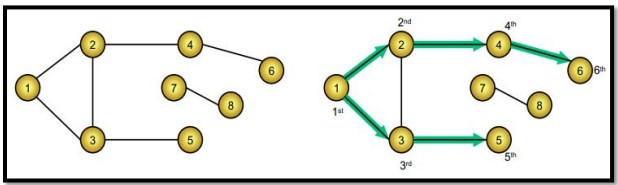
\includegraphics[width=0.8\textwidth]{
		Figures/figs/bieuDienCayBFS.jpg
	}
	\caption[Biểu diễn cây BFS]{
		Biểu diễn cây BFS
	}
	\label{fig:hinhd}
\end{figure}

\textbf{Ưu điểm}
\begin{itemize}
	\item Kỹ thuật tìm kiếm rộng là kỹ thuật vét cạn không gian trạng thái bài toán vì
	vậy sẽ tìm được lời giải nếu có
	\item Đường đi tìm được thỏa mãn đi qua ít đỉnh nhất.
\end{itemize}

\textbf{Nhược điểm}
\begin{itemize}
	\item Tìm kiếm lời giải theo thuật toán đã định trước, do vậy tìm kiếm một cách
	máy móc; khi không có thông tin bổ trợ cho quá trình tìm kiếm, không nhận
	ra ngay lời giải.
	\item Không phù hợp với không gian bài toán có kích thước lớn. Đối với loại bài
	toán này thì phương pháp tìm kiếm chiều rộng đối diện với các khó khăn về
	nhu cầu:
		\subitem - Cần nhiều bộ nhớ theo số nút cần lưu trữ.
		\subitem - Cần nhiều công sức xử lý các nút, nhất là khi các nhánh cây dài, số
		nút tăng.
		\subitem - Dễ thực hiện các thao tác không thích hợp , thừa, đưa đến việc tăng
		đáng kể số nút phải xử lý.
	\item Không hiệu quả nếu lời giải ở sâu. Phương pháp này không phù hợp cho
	trường hợp có nhiều đường dẫn đến kết quả nhưng đều sâu.
	\item Giao tiếp với người dùng không thân thiện. Do duyệt qua tất cả các nút,
	việc tìm kiếm không tập trung vào một chủ đề.
\end{itemize}

\section{Độ phức tạp của BFS và DFS}
Quá trình tìm kiếm trên đồ thị bắt đầu từ một đỉnh có thể thăm tất cả các đỉnh còn
lại, khi đó cách biểu diễn đồ thị có ảnh hưởng lớn tới chi phí về thời gian thực hiện
giải thuật:
\begin{itemize}
	\item Trong các trường hợp ta biểu diễn đồ thị bằng danh sách kề, cả hai thuật
	toán BFS và DFS đều có độ phức tạp tính toán là O(n+m) = O(max(n,m)).
	Đây là cách cài đặt tốt nhất.
	\item Nếu ta biểu diễn đồ thị bằng ma trận kề thì độ phức tạp tính toán trong
	trường hợp này là $O(n+n^2) = O(n^2).$
	\item Nếu ta biểu diễn đồ thị bằng danh sách cạnh, thao tác duyệt những đỉnh kề
	với đỉnh u sẽ dẫn tới việc duyệt toàn bộ danh sách cạnh, đây là cách cài đặt
	tồi tệ nhất, nó có độ phức tạp tính toán là O(n.m).
\end{itemize}





 
% Chương 3

\chapter{KẾT QUẢ} % Tên của chương

\label{Chapter3} % Để trích dẫn chương này ở chỗ nào đó trong bài, hãy sử dụng lệnh \ref{Chapter3} 

%----------------------------------------------------------------------------------------

\section{Giao diện}

\begin{figure}[h!]
	\centering
	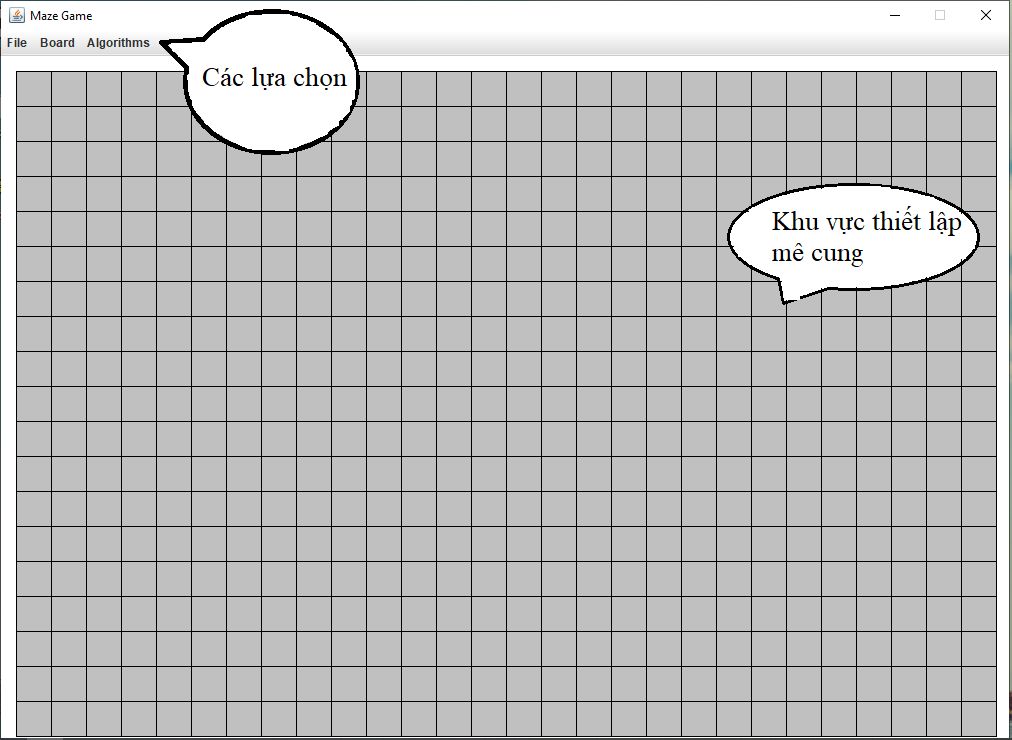
\includegraphics[width=0.8\textwidth]{
		Figures/figs/1.PNG
	}
	\caption[Giao diện game với phần tạo mê cung và các lựa chọn]{
		Giao diện game với phần tạo mê cung và các lựa chọn 
	}
	\label{fig:hinhe}
\end{figure}


\begin{figure}[h!]
	\centering
	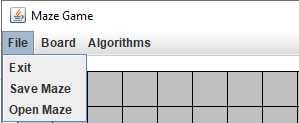
\includegraphics[width=0.8\textwidth]{
		Figures/figs/2.PNG
	}
	\caption[Chức năng lựa chọn File]{
		Chức năng lựa chọn File 
	}
	\label{fig:hinhf}
\end{figure}

Chức năng lựa chọn \textbf{File}:
\begin{itemize}
	\item Exit: Thoát khỏi trò chơi
	\item Save Maze: Lưu lại mê cung đã tạo vào máy
	\item Open Maze: Mở một mê cung đã có sẵn.
\end{itemize}

\begin{figure}[h!]
	\centering
	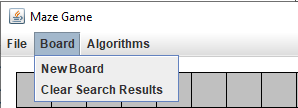
\includegraphics[width=0.8\textwidth]{
		Figures/figs/3.PNG
	}
	\caption[Chức năng lựa chọn Board:]{
		Chức năng lựa chọn Board: 
	}
	\label{fig:hinhg}
\end{figure}

Chức năng lựa chọn \textbf{Board}:
\begin{itemize}
	\item New Board: Tạo một giao diện trò chơi mới
	\item Clear Search Result: Xóa đường đi thuật toán đã tìm kiếm
\end{itemize}

\begin{figure}[h!]
	\centering
	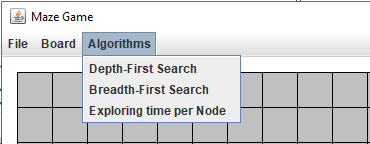
\includegraphics[width=0.8\textwidth]{
		Figures/figs/4.PNG 
	}
	\caption[Chức năng lựa chọn Algorithms]{
		Chức năng lựa chọn Algorithms 
	}
	\label{fig:hinhh}
\end{figure}

Chức năng lựa chọn \textbf{Algorithms}:
\begin{itemize}
	\item Depth-First Search: Sử dụng thuật toán DFS
	\item Breadth-First Search: Sử dụng thuật toán BFS
	\item Exploring time per Node: Cài đặt thời gian
\end{itemize}

\begin{figure}[h!]
	\centering
	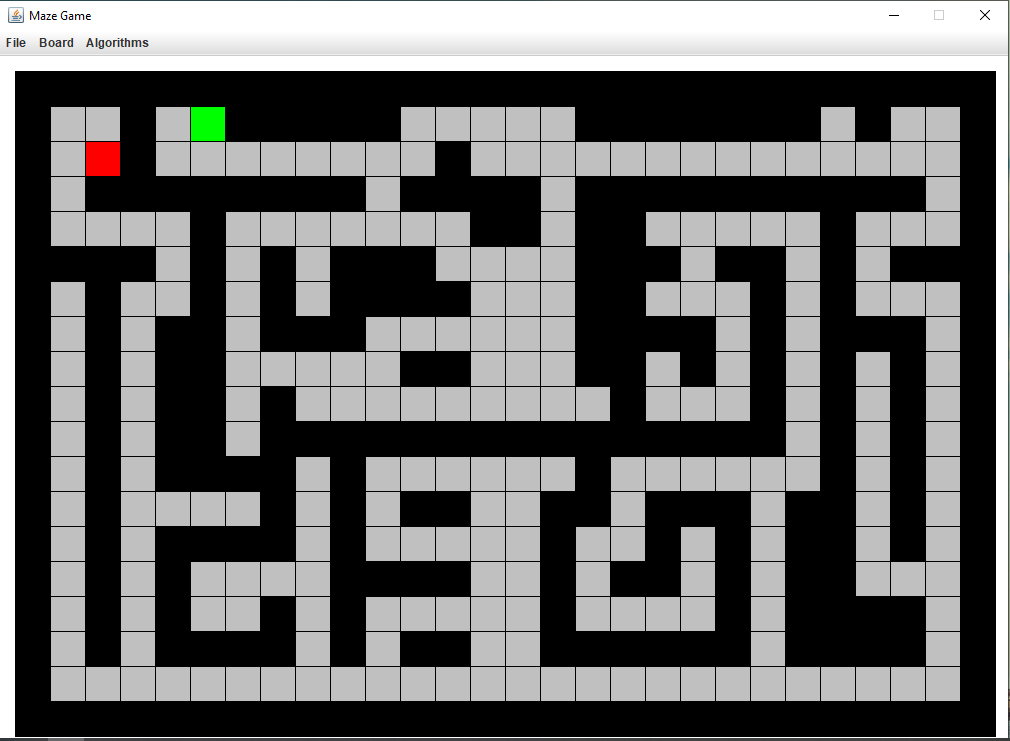
\includegraphics[width=0.7\textwidth]{
		Figures/figs/5.PNG
	}
	\caption[Giao diện mê cung đã được thiết lập với các thông tin]{
		Giao diện mê cung đã được thiết lập với các thông tin	 
	}
	\label{fig:hinhi}
\end{figure}

Giao diện mê cung đã được thiết lập với các thông tin:
\begin{itemize}
	\item Ô màu đen: Tường, chướng ngại vật không thể di chuyển qua được
	\item Ô màu xám: Vị trí có thể đi qua
	\item Ô màu đỏ: Vị trí đích
	\item Ô màu xanh: Vị trí bắt đầu
\end{itemize}

\newpage
\section{Kết quả}
\subsection{Thuật toán DFS}
\begin{figure}[h!]
	\centering
	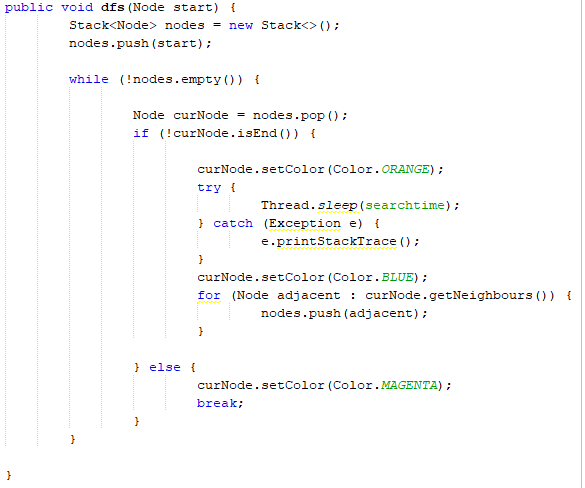
\includegraphics[width=0.8\textwidth]{
		Figures/figs/8.PNG
	}
	\caption[Thuật toán DFS tìm kiếm đường đi theo chiều sâu]{
		Thuật toán DFS tìm kiếm đường đi theo chiều sâu
	}
	\label{fig:hinhK}
\end{figure}

Trong đó:
\begin{enumerate}
	\item Tạo một đối tượng 'Stack<Node>' để lưu trữ các nút chưa được duyệt trong quá trình tìm kiếm.
	\item Đưa nút 'start' vào 'Stack' và bắt đầu vòng lặp while khi 'Stack' chưa rỗng.
	\item Lấy ra nút đầu tiên trong 'Stack' dùng 'pop()'
	\item Kiểm tra nếu nút hiện tại là nút đích ('isEnd()') thì đổi màu thành màu Magenta và dừng thuật toán.
	
	\item Nếu nút không phải đích, đổi màu thành màu cam và ngủ trong một khoảng thời gian (tùy chọn).
	\item Đổi màu của nút về màu xanh dương và thêm các nút kề vào 'Stack'.
	\item Lặp lại từ bước 3.
	\item Khi thuật toán kết thúc, đường đi từ nút bắt đầu đến nút đích sẽ được tô màu Magenta.
\end{enumerate}

\begin{figure}[h!]
	\centering
	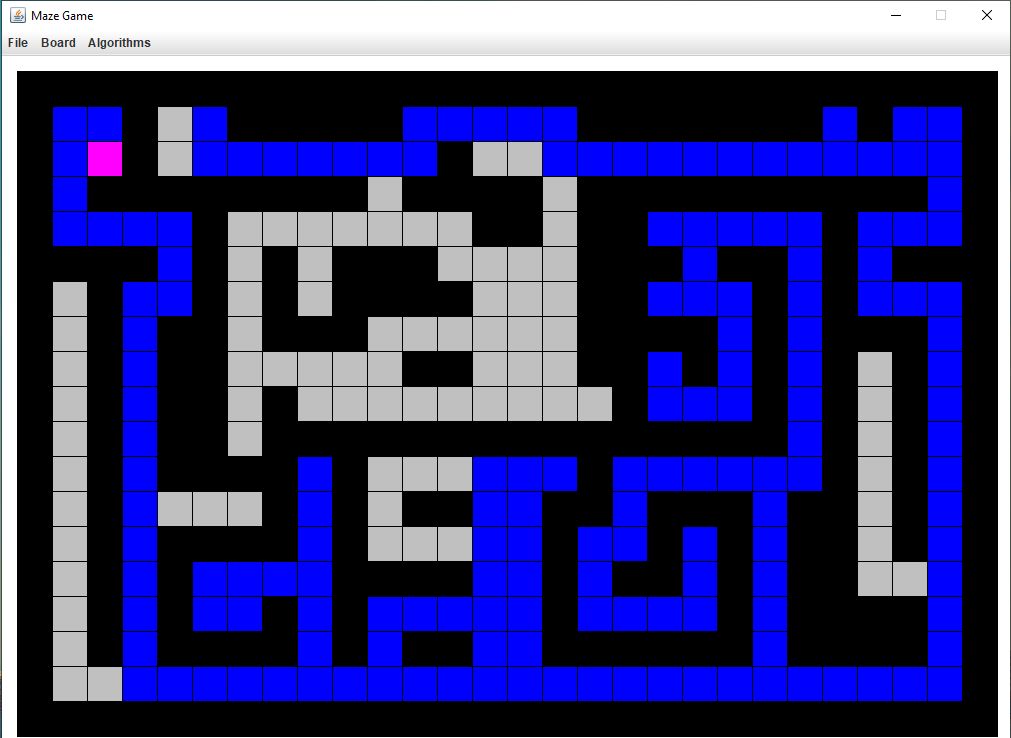
\includegraphics[width=0.8\textwidth]{
		Figures/figs/6.PNG
	}
	\caption[Kết quả tìm kiếm đường đi ma trận bằng thuật toán DFS]{
		Kết quả tìm kiếm đường đi ma trận bằng thuật toán DFS
	}
	\label{fig:hinhl}
\end{figure}

\newpage
\subsection{Thuật toán BFS}
\begin{figure}[h!]
	\centering
	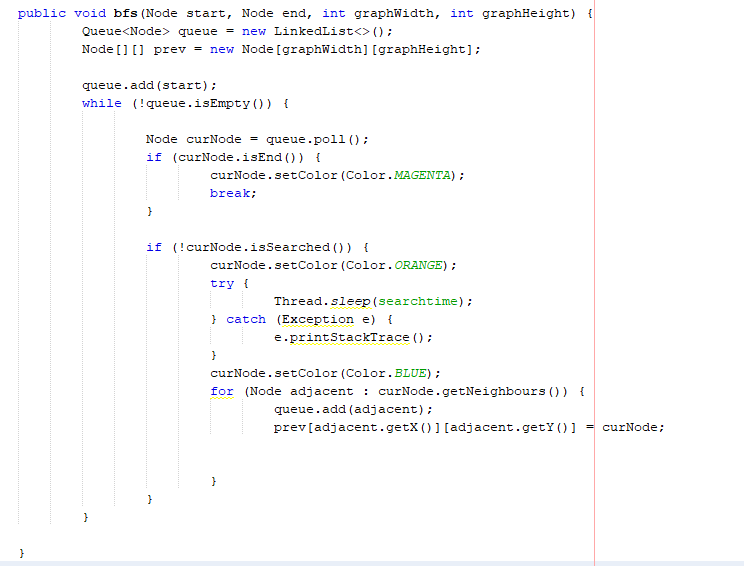
\includegraphics[width=0.8\textwidth]{
		Figures/figs/9.PNG
	}
	\caption[Thuật toán BFS tìm kiếm đường đi theo chiều rộng]{
		Thuật toán BFS tìm kiếm đường đi theo chiều rộng 
	}
	\label{fig:hinhm}
\end{figure}

Trong đó:
\begin{enumerate}
	\item Tạo một 'Queue<Node>' để lưu trữ các nút chưa được duyệt.
	\item Khởi tạo một mảng 2 chiều 'Node[][]' để lưu trữ nút đi trước của nút hiện tại.
	\item Thêm nút 'start' vào hàng đợi ('queue') và bắt đầu vòng lặp while khi hàng đợi chưa rỗng.
	\item Lấy nút đầu tiên ra khỏi hàng đợi dùng 'poll()'.
	\item Nếu nút là nút đích ('isEnd()'), thì đổi màu của nút thành Magenta, và kết thúc thuật toán.
	\item Nếu nút chưa được tìm kiếm, thì đổi màu thành Orange và ngủ một khoảng thời gian tùy chọn.
	\item Đổi màu của nút về màu Blue và thêm các nút kề của nó vào hàng đợi ('queue').
	\item Lưu trữ nút đóng vai trò là nút đi trước của nút hợp lệ trong mảng prev dựa trên vị trí hàng và cột của nút trong đồ thị.
	\item Lặp lại từ bước 4.
	\item Khi thuật toán kết thúc, tìm đường đi ngắn nhất từ nút 'start' đến nút 'end' sử dụng mảng 'prev' và sắp xếp các nút trên đường đi này thành màu Magenta.
\end{enumerate}

\begin{figure}[h!]
	\centering
	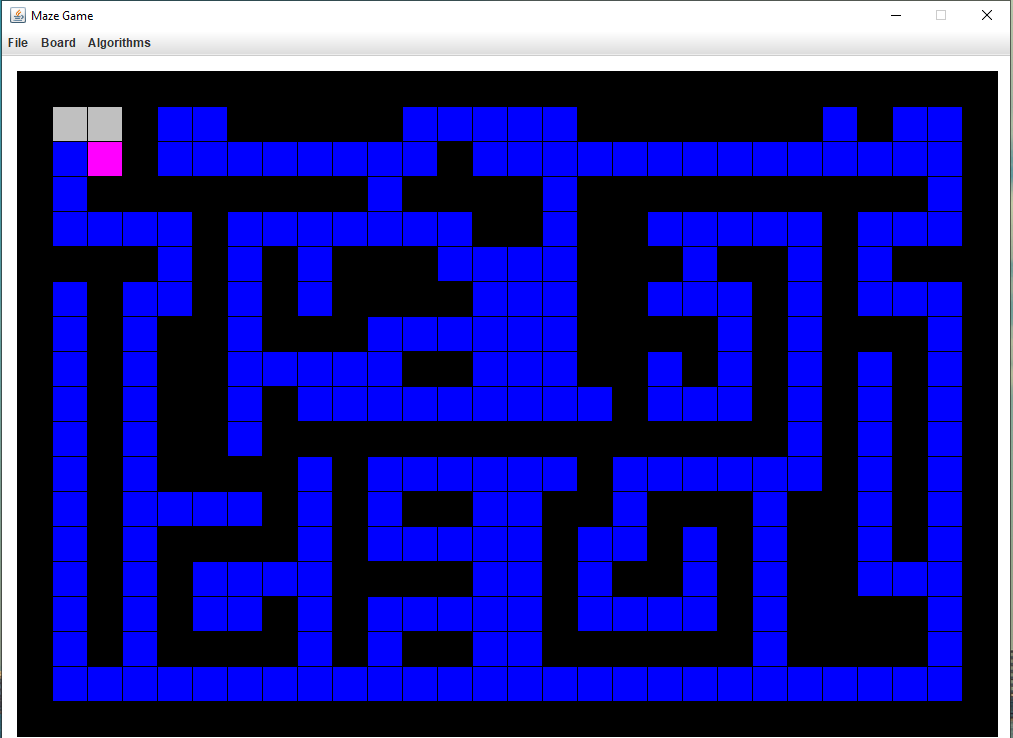
\includegraphics[width=0.6\textwidth]{
		Figures/figs/7.PNG
	}
	\caption[Kết quả tìm kiếm đường đi ma trận bằng thuật toán BFS]{
		Kết quả tìm kiếm đường đi ma trận bằng thuật toán BFS
	}
	\label{fig:hinhn}
\end{figure}


 
%% Chương 4
\chapter{KẾT QUẢ} % Tên của chương

\label{Chapter4} % Để trích dẫn chương này ở chỗ nào đó trong bài, hãy sử dụng lệnh \ref{Chapter4}

\begin{figure}[h!]
	\centering
	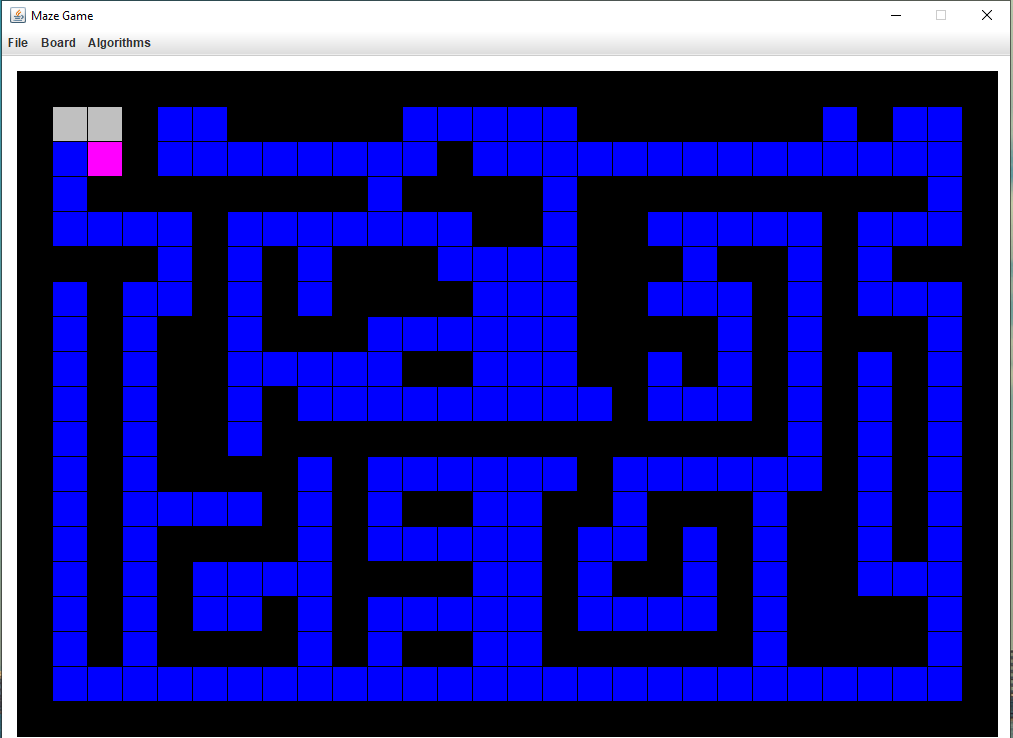
\includegraphics[width=0.4\textwidth]{
		Figures/figs/7.png
	}
	\caption[Trạng thái ban đầu]{
		Trạng thái ban đầu
	}
	\label{fig:hinh8}
\end{figure}

Với trạng thái bắt đầu là trạng thái ở hình trên, ta có kết quả thực hiện tương ứng với các thuật toán.

\newpage
\section{Kết quả thuật toán BFS}
\begin{figure}[h!]
	\centering
	\includegraphics[width=0.5\textwidth]{
		Figures/figs/BFS.jpg
	}
	\caption[Kết quả thuật toán BFS]{
		Kết quả thuật toán BFS
	}
	\label{fig:hinh11}
\end{figure}

Số bước đi = 4

Số phép toán đã thực hiện = 30

Thời gian tính toán = 0.015s


\newpage
\section{Kết quả thuật toán DFS}
\begin{figure}[h!]
	\centering
	\includegraphics[width=0.5\textwidth]{
		Figures/figs/DFS.jpg
	}
	\includegraphics[width=0.5\textwidth]{
		Figures/figs/DFS_2.jpg
	}
	\caption[Kết quả thuật toán DFS]{
		Kết quả thuật toán DFS
	}
	\label{fig:hinh12}
\end{figure}

%\begin{figure}[h!]
%	\centering
%	\includegraphics[width=0.5\textwidth]{
%		Figures/figs/DFS_2.jpg
%	}
%	\caption[Kết quả thuật toán DFS 2]{
%		Kết quả thuật toán DFS 2
%	}
%	\label{fig:hinh15}
%\end{figure}

%\newpage
Chi phí tối đa của thuật toán = 15

Số bước đi = 8

Số phép toán đã thực hiện = 3244

Thời gian tính toán = 0.047s






\chapter*{KẾT LUẬN} % Tên của chương
\addcontentsline{toc}{chapter}{KẾT LUẬN} % Thêm tên chương vào mục lục

\label{Chapter5} % Để trích dẫn chương này ở chỗ nào đó trong bài, hãy sử dụng lệnh \ref{Chapter0} 

%----------------------------------------------------------------------------------------

Thông qua việc tìm hiểu và nghiên cứu về đề tài này giúp chúng em có cái nhìn toàn diện hơn trong việc ứng dụng thuật toán tìm kiếm trong đồ thị tìm kiếm đường đi trong mê cung. Bài toán tìm kiếm đường đi trong mê cung là chủ đề đã được nhiều người nghiên cứu giải quyết nhưng cho đến nay vẫn chưa có cách giải quyết tối ưu cho tất cả trạng thái. Hy vọng việc áp dụng thuật toán tìm kiếm trong đồ thị sẽ góp phần bổ sung thêm một hướng giải quyết cho bài toán. Do thời gian có hạn nên đề tài không tránh khỏi sai sót, mong thầy góp ý, đánh giá giúp chúng tôi hoàn thiện đề tài
 

%----------------------------------------------------------------------------------------
%	(KHÔNG CHỈNH SỬA PHẦN NÀY)
%
%	PHẦN 13: TÀI LIỆU THAM KHẢO
%----------------------------------------------------------------------------------------

\begin{spacing}{1.15}
	\printbibliography[heading=bibintoc, title=Tài liệu tham khảo] % In ra tài liệu tham khảo
	
\end{spacing}

%----------------------------------------------------------------------------------------
%	PHẦN 14: PHỤ LỤC (THESIS CONTENT - APPENDICES)
%----------------------------------------------------------------------------------------

\appendix % Nói với LaTeX rằng những chương về sau được tính là phụ lục

% Hãy thêm những phụ lục (appendix) của khóa luận/tiểu luận vào thư mục Appendices
% Hãy bỏ chú thích những dòng nếu bạn đã bổ sung những phụ lục vào

%% Phụ lục B

\chapter{Chương trình chính - điều chế độ rộng xung pwm phụ thuộc vào biến trở} % Tên của phụ lục

\label{AppendixA} % Để trích dẫn chương này ở chỗ nào đó trong bài, hãy sử dụng lệnh \ref{AppendixA} 

%----------------------------------------------------------------------------------------

%\begin{Verbatim}
%\lstinputlisting{"Code/TieuLuan.c"}
%\end{Verbatim}

%https://www.programiz.com/cpp-programming/examples/time-structure
\lstinputlisting{"Code/baiTapCuoiKy.c"}


%----------------------------------------------------------------------------------------


%% Phụ lục B

\chapter{Chương trình chính - Điều chế độ rộng xung pwm} % Tên của phụ lục

\label{AppendixB} % Để trích dẫn chương này ở chỗ nào đó trong bài, hãy sử dụng lệnh \ref{AppendixB} 

%----------------------------------------------------------------------------------------

%\begin{Verbatim}
%\lstinputlisting{"Code/TieuLuan.c"}
%\end{Verbatim}

%https://www.programiz.com/cpp-programming/examples/time-structure
\lstinputlisting{"Code/baiTapCuoiKy2.c"}


%----------------------------------------------------------------------------------------


%\include{Appendices/AppendixC}

%----------------------------------------------------------------------------------------

\end{document} 
%----------------------------------------------------------------------------------------------------------------------------------------
